\lecture{20}{13. November 2025}{Statically Indeterminate Beams}

\subsection{Statically Indeterminate Beams and Shafts -- Method of Superposition}
In order to use the method of superposition to solve for the reactions on a statically indeterminate beam, we must first identify the redundants and remove them from the beam.
The will produce the \textit{primary beam}, which will be statically determinate and stable.
Using superposition, we add a succession of similarly supported beams, each loaded with a separate redundant to the primary beam.
The redundants may be determined from the \textit{conditions of compatibility} that exist at each support where a redundant acts.

\begin{figure} [ht]
  \centering
  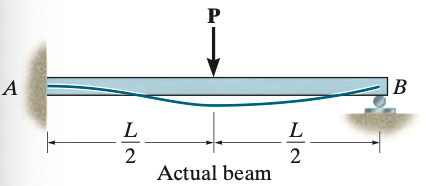
\includegraphics[width=0.8\linewidth]{./figures/f16_23a.png}
  \caption{}
  \label{fig:f16_23a}
\end{figure}

To clarify, consider the beam depicted on \Cref{fig:f16_23a}.
If we choose the reaction $\Vec{B}_y$ at the roller as our redundant, then the primary beam becomes as shown on \Cref{fig:f16_23b} and the beam with only the redundant $\Vec{B}_y$ acting on it is shown on \Cref{fig:f16_23c}.
The displacement at the roller is set to be zero, and since the displacement of $B$ on the primary beam is $v_B$ and $\Vec{B}_y$ causes $B$ to be displaced upward $v'_B$, we can write the compatibility equation as:
\begin{equation*}
  0 = - v_B + v_B'
.\end{equation*}
These displacements can be expressed in terms of the loads using the table in Appendix D of the book.
These load-displacement relations are
\begin{equation*}
  v_B = \frac{5 PL^3}{48 EI} \qquad v_B' = \frac{B_y L^3}{3EI}
.\end{equation*}
Substituting these into the compatibility equations we get
\begin{gather*}
  0 = - \frac{5 PL^3}{48 EI} + \frac{B_y L^3}{3 EI} \\
  B_y = \frac{5}{16}P
.\end{gather*}

\begin{figure} [ht]
  \centering
  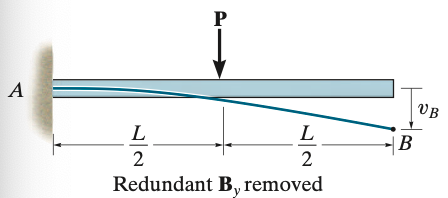
\includegraphics[width=0.8\linewidth]{./figures/f16_23b.png}
  \caption{}
  \label{fig:f16_23b}
\end{figure}

\begin{figure} [ht]
  \centering
  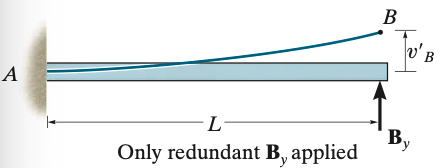
\includegraphics[width=0.8\linewidth]{./figures/f16_23c.png}
  \caption{}
  \label{fig:f16_23c}
\end{figure}

Now that $\Vec{B}_y$ is known, the reactions at the wall can be determined from the equilibrium equations.
The choice of the redundant is arbitrary, provided the beam remains stable -- e.g. the moment at $A$ on \Cref{fig:f16_23a} could also have been chosen as a redundant.
